\title{Lab Assignment 1 \\ \small{Datamining}}
\author{Chiel ten Brinke 3677133}
\documentclass[12pt]{article}
\usepackage{amssymb,amsmath,amsthm,enumerate,graphicx,float,lmodern}

\newtheorem{theorem}{Theorem}[section]
\newtheorem{lemma}[theorem]{Lemma}
\newtheorem{proposition}[theorem]{Proposition}
\newtheorem{corollary}[theorem]{Corollary}

\theoremstyle{definition}
\newtheorem{definition}[theorem]{Definition}
\newtheorem{axiom}[theorem]{Axiom}
\newtheorem{example}[theorem]{Example}
\newtheorem{remark}[theorem]{Remark}

\newcommand{\set}[2]{\left\lbrace#1 \, \middle|\, #2 \right\rbrace}

\begin{document}
\maketitle

\section{Data Set}
\label{sec:dataset}

The data set that has been used for this assignment is called Covertype Data Set and has been
taken from the UCI machine learning
repository\footnote{http://archive.ics.uci.edu/ml/data sets/Covertype}.
There are 55 attributes, which is relatively many.
Some first tests showed that the data set was very predictable.
Therefore, to make the results less trivial, we shall disregard some attributes.
Besides the fact that there are many attributes, there are also a lot of data instances
($> 500 000$).
Because this amount of data leads to inconvenient running times, and because of the
predictability of the data set, we shrinked the data set (in a randomized manner)
down to a size that is more suitable for this assignment.
The resulting data set contains $10000$ instances.

The training set and test set are sampled randomly from the data set, such that
they are complementary and have ratio 7:3 as required.

As classlabel column 13 is used, and as attributes columns 1 till 10 are used.
This is because column 13 is the binary label where the number 0's and 1's are most
equally distributed, whereas most of the other binary labels are very unequally distributed,
giving trivial results.

\section{Finding good parameter values}
\label{sec:finding}

In order to find good values for nmin and minleaf, i.e.\ those that result in a low error rate,
a plot has been made of the behaviour of the error rate as a function of nmin and minleaf.
To keep the compution time within reasonable bounds, the values for nmin and minleaf were
tested on random samples from the data set of size 100.
The resulting plots are shown in Figure~\ref{fig:graph1} and Figure~\ref{fig:graph2}.

\begin{figure}[H]
    \centering
    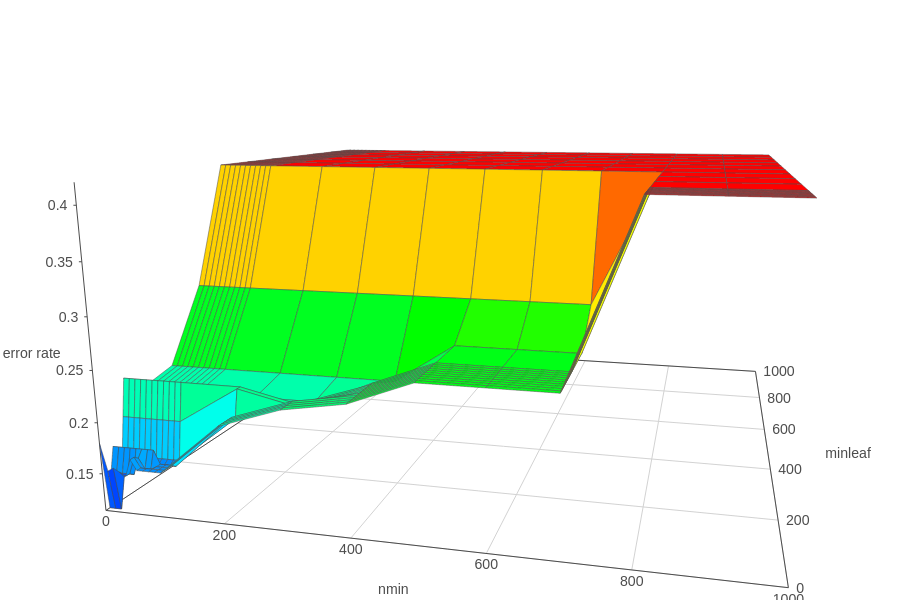
\includegraphics[width=0.8\linewidth]{graph1.png}
    \caption{Error rate as a function of nmin and minleaf.}
\label{fig:graph1}
\end{figure}

\begin{figure}[H]
    \centering
    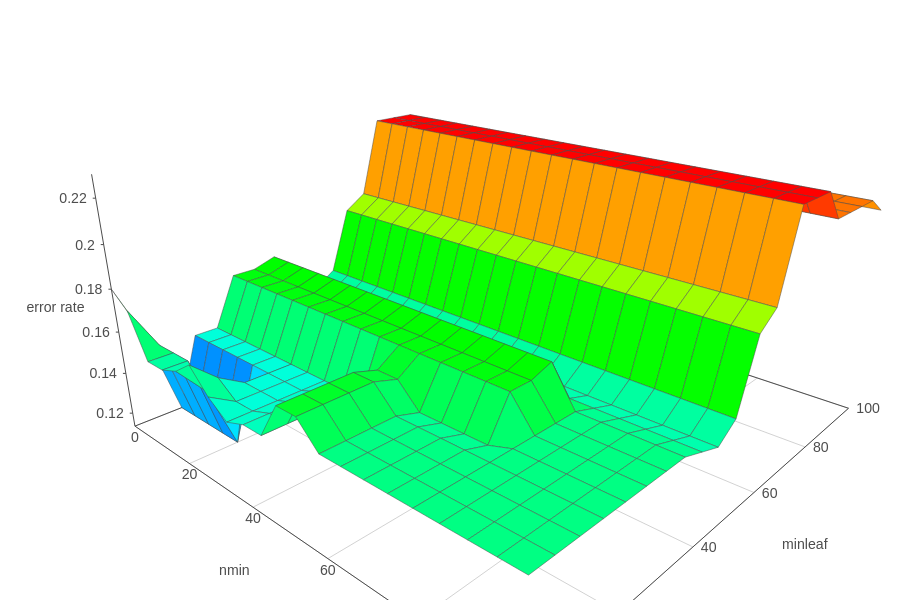
\includegraphics[width=0.8\linewidth]{graph2.png}
    \caption{Error rate as a function of nmin and minleaf.}
\label{fig:graph2}
\end{figure}


It is likely that the error rate will not behave exactly the same when evaluated on
the entire data set instead of a very small sample.
Nonetheless, as one can see, the graphs do give a clue that choosing low values
for nmin and minleaf works best for this dataset.

\section{Results}
\label{sec:results}

Taking into account that low values for nmin and minleaf probably work best,
various configurations on the entire data set have been tested
as shown in Table~\ref{table1}

\begin{table}[h]
\centering
\begin{tabular}{lll}
    nmin & minleaf & error rate \\
    \hline \hline
    1 & 1  & 0.0966667 \\
    2 & 1  & 0.0966667 \\
    3 & 1  & 0.0963333 \\
    4 & 1  & 0.099 \\
    5 & 1  & 0.09833333 \\
    1 & 2  & 0.1006667 \\
    2 & 2  & 0.1006667 \\
    3 & 2  & 0.1006667 \\
    4 & 2  & 0.1006667 \\
    5 & 2  & 0.1013333 \\
    10 & 5  & 0.109 \\
    20 & 5  & 0.1136667 \\
    30 & 5  & 0.11433 \\
    20 & 10 & 0.119 \\
    50 & 10 & 0.112333 \\
    100 & 50 & 0.1196667 \\
    %20 & 1  & 0.1086667 \\
    %30 & 1  & 0.107333 \\
\end{tabular}
\caption{Error rate as function of nmin and minleaf tested on the entire dataset.}
\label{table1}
\end{table}

Note that $\mathrm{nmin} = 3$ and $\mathrm{minleaf} = 1$ resulted in the lowest error rate.
This is a remarkably low configuration.
On one hand this suggests again that this data set is very consistent and predictable,
without much random scatter such that overfitting can hardly occur.
On the other hand we see that the error rate is still about $10\%$, so since there is presumably
not much random scatter, there is probably contradictory data present in the data set.
In Table~\ref{table2} one can see the corresponding confusion matrix.

\begin{table}[h]
\centering
\begin{tabular}{r||ll}
     & 0    & 1   \\
    \hline \hline
    0 & 1723 & 154 \\
    1 & 135  & 980 \\
\end{tabular}
\caption{Confusion matrix for $\mathrm{nmin} = 3$ and $\mathrm{minleaf} = 1$.}
\label{table2}
\end{table}

\end{document}
